\documentclass{standalone}

\usepackage{tikz,amsmath,amssymb,bm,color}
\usetikzlibrary{shapes,arrows,arrows.meta}
% needed for BB
\usetikzlibrary{patterns}
\usetikzlibrary{fit}
\usetikzlibrary{calc,3d}

\pgfdeclareimage[width=1.6cm]{x10}{./matlab/X10.png}
\pgfdeclareimage[width=8mm]{x20}{./matlab/X20.png}
\pgfdeclareimage[width=8mm]{x10d}{./matlab/X10.png}
\pgfdeclareimage[width=4mm]{x20d}{./matlab/X20.png}
%\pgfdeclareimage[width=1.6cm]{x20u}{./matlab/X20.png}
\pgfdeclareimage[width=1.6cm]{x20u}{./matlab/pred.png}


\tikzstyle{FRAME}=[rectangle,draw,ultra thick, minimum width=1.6cm, minimum height=1.6cm,inner sep=0pt]
\tikzstyle{Frame}=[rectangle,draw, ultra thick,minimum width=0.8cm, minimum height=0.8cm,inner sep=0pt]
\tikzstyle{frame}=[rectangle,draw,very thick, minimum width=0.4cm, minimum height=0.4cm,inner sep=0pt]

\definecolor{col10}{rgb}{0,0.5,0.8}%{0.2, 0.5, 1}
\definecolor{col20}{rgb}{0.8,0.2,0.0}%{0.2, 0.5, 1}%{1, 0.2, 0.2}
\definecolor{colLoss}{rgb}{0.8,0.8,0.2}%{0.2, 0.5, 1}%{1, 0.2, 0.2}

\tikzstyle{BOX}=[rectangle,dashed, draw,minimum width=2.1cm, minimum height=0.8cm,inner sep=0pt]
\tikzstyle{LPF}=[rectangle, draw,minimum width=0.8cm, minimum height=0.4cm,inner sep=0pt]
\tikzstyle{DWN}=[rectangle, draw,minimum width=0.4cm, minimum height=0.4cm,inner sep=0pt]
\tikzstyle{CNN}=[rectangle,draw, very thick, minimum width=1.2cm, minimum height=0.6cm,inner sep=0pt]
\tikzstyle{DET}=[rectangle,draw, thick, minimum width=1.2cm, minimum height=0.6cm,inner sep=1pt]


\tikzstyle{Loss}=[circle, fill=colLoss, very thick,draw, minimum size=0.8cm, inner sep=0pt]
\tikzstyle{SUM}=[circle, thick,draw, minimum size=0.3cm, inner sep=0pt]
\tikzstyle{arr}=[thick, -stealth]


\begin{document}

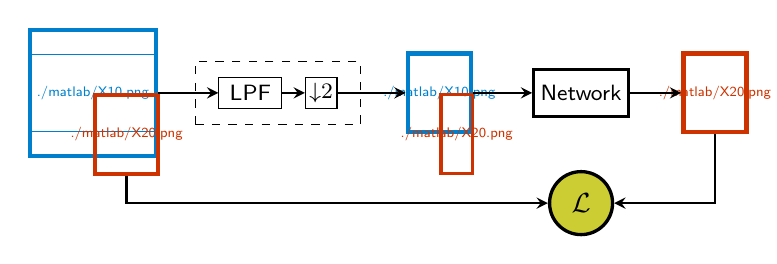
\begin{tikzpicture}[node distance=2cm]
\sf

\node[coordinate](O) at (0,0){}; % origine
\node[FRAME,col10](I1) at (0,0){\pgfuseimage{x10}}; 
\node[Frame,col20,anchor=north west](I2) at (0,0){\pgfuseimage{x20}}; 

\node[LPF, right of=I1,font=\footnotesize](lpf) {LPF};
\node[DWN, right of=lpf, node distance = 0.9cm,font=\footnotesize](down) {${\downarrow}2$};
\node[BOX, right of=I1,xshift = 3.5mm,font=\footnotesize](Down) {};

\node[Frame,col10,right of=down, xshift=-5mm](R1) {\pgfuseimage{x10d}}; 
\node[frame,col20,anchor=north west](R2) at (R1){\pgfuseimage{x20d}}; 

\node[CNN, right of=R1,font=\footnotesize,xshift=-2mm](net) {Network};

\node[Frame,col20,right of = net,xshift=-3mm](pred) {\pgfuseimage{x20}};

\node[Loss, below of=net, node distance = 1.4cm](loss) {$\mathcal{L}$};

\draw[arr] (I1)--(lpf);  \draw[arr] (lpf)--(down); \draw[arr] (down)--(R1); \draw[arr] (R1)--(net); \draw[arr] (net)--(pred); 

\draw[arr] (I2)|-(loss);
\draw[arr] (pred)|-(loss);


\end{tikzpicture}

\end{document}